\section{Supplementary studies}\label{app:studies}

This appendix reports the two studies summarized in Section~\ref{sec:exp} and the
granularity, score and cell-size sensitivity analyses referred to there. Each applies the
estimator of Section~\ref{sec:method} without modification; only the declared grouping
variable $\phi$ changes.

\subsection{Sensitivity analyses}\label{sec:ablations}

For MLP-SPATIAL versus MLP-CLASS, the conclusion survives every planned sensitivity
check (Table~\ref{tab:sensitivity}). Changing from the quadratic to a probability-floored
log score changes scale ($0.01439$ to $0.06536$) but not sign or significance.
The coverage column matters for reading the rows against each other, and earlier
versions of this table omitted it. Each row targets the identified subpopulation its own
setting defines, so the minimum-cell-size rows are not four estimates of one quantity:
raising the minimum from $2$ to $20$ drops coverage from $99.0\%$ to $86.7\%$ and changes
the estimand along with the estimator. That the estimate moves so little across them
($0.01439$ to $0.01225$) is therefore mild evidence of stability rather than a
sensitivity analysis holding the target fixed.

Coarsening $\phi$ from the class pair to subject class increases the credited covariance
to $0.02181$. Proposition~\ref{prop:coarsen} identifies why: the coarser cell's estimate
equals the class-pair estimate's conditional average plus a between-class-pair covariance
term, and that term is positive here, meaning some of the credited gain reflects
class-pair-level structure that the finer audit had already correctly assigned to
$\Delta P$. This is precisely the sense in which the class-pair audit is the conservative
choice: it is not that coarsening is wrong, but that it cannot be assumed neutral, and
only the finer partition's estimate isolates covariance gain net of every prior regularity
expressible in $\phi$. The same class-pair-versus-subject-only pair also instantiates
Proposition~\ref{prop:sensitivity} directly, with the subject class playing the role of
the unrecorded confounder $Z$: Table~\ref{tab:sensitivity-numeric} in
Section~\ref{sec:sensitivity} reports that the resulting bias of $0.00742$ is comfortably
inside the Cauchy--Schwarz bound, though the bound is loose enough at $K=50$ that it
would remain satisfied for a $\bar\rho$ three orders of magnitude smaller than one.
Raising the minimum cell size from 2 to 5, 10, and 20 yields
$0.01395$, $0.01330$, and $0.01225$; all cluster-robust lower limits remain positive.
The procedure itself has no smoothing strength, split fraction, or decision threshold
to tune.

\begin{table}[t]
\centering
\caption{Sensitivity of the MLP-SPATIAL vs.\ MLP-CLASS decomposition to score, audit
granularity, and minimum cell size. CI is image-cluster robust on $\widehat{\Delta R}$.}
\label{tab:sensitivity}
\small
\begin{tabular}{@{}llrr@{\,}rr@{}}
\toprule
Factor & Setting & $\widehat{\Delta T}$ & \multicolumn{1}{r}{$\widehat{\Delta R}$ (95\% CI)} & Cells &
Cov. \\
\midrule
Score & Brier (def.) & $0.00885$ & $0.01439\,[0.01373,0.01504]$ & 6346 & $99.0\%$ \\
Score & Log (floored) & $0.04297$ & $0.06536\,[0.06294,0.06779]$ & 6346 & $99.0\%$ \\
Cell $\phi$ & class pair (def.) & $0.00885$ & $0.01439\,[0.01373,0.01504]$ & 6346 & $99.0\%$ \\
Cell $\phi$ & subject only & $0.00943$ & $0.02181\,[0.02079,0.02283]$ & 150 & $100.0\%$ \\
Min.\ cell size & 2 (def.) & $0.00885$ & $0.01439\,[0.01373,0.01504]$ & 6346 & $99.0\%$ \\
Min.\ cell size & 5 & $0.00772$ & $0.01395\,[0.01329,0.01462]$ & 4060 & $96.3\%$ \\
Min.\ cell size & 10 & $0.00683$ & $0.01330\,[0.01262,0.01398]$ & 2744 & $92.6\%$ \\
Min.\ cell size & 20 & $0.00570$ & $0.01225\,[0.01155,0.01295]$ & 1757 & $86.7\%$ \\
\bottomrule
\end{tabular}
\end{table}


\subsection{Long-tailed image classification}\label{app:lt}\label{sec:cifarlt}

Sections~\ref{app:vgmain}--\ref{app:vgvisual} are all instances of one task (predicate
classification on an ordered object pair). Section~\ref{sec:related-applied} argued
that long-tailed image classification poses a structurally identical question: a
class-frequency prior can be fit better without any per-instance improvement. We test
this directly on CIFAR-100-LT \citep{cui2019classbalanced}, an exponential-imbalance
(ratio $100$) subsample of CIFAR-100's training split with the original, balanced test
split retained for evaluation. We train ResNet-32 \citep{he2016deep} classifiers that
differ only in their per-class loss weighting: a vanilla cross-entropy baseline (CE);
class-balanced effective-number re-weighting applied from initialization (CB)
\citep{cui2019classbalanced}; and the same re-weighting deferred to the final twenty
epochs (DRW) \citep{cao2019learning}. Optimizer, schedule, augmentation, epoch budget,
and seed are identical across runs (Appendix~\ref{app:implementation}).

\paragraph{Choosing $\phi$.} A declared grouping variable has to predict the label without
determining it, and this second benchmark makes the constraint unusually easy to
violate. Were $\phi$ taken to be the fine class label itself, every cell would be
label-homogeneous, within-cell transport would have nothing to cross, and
$\widehat{\Delta R}$ would come out identically zero -- an algebraic artifact wearing the
appearance of a finding. CIFAR-100's own 20 coarse superclasses avoid this, each
gathering five fine labels into a cell of $500$ balanced test images, which is
structurally the situation of a VG class-pair cell holding several predicates
(Figure~\ref{fig:samples}). Alongside the superclass audit we report two further
declared priors: the trivial coarsening to a single global cell, which audits against
the global class marginal and so instantiates Proposition~\ref{prop:coarsen} in a second
domain, and a partition into head, medium and tail training-frequency tiers. CIFAR-100
test images are independent, unlike the several relations VG draws from one photograph,
so no cluster grouping is required and the plain H\'ajek interval of
Section~\ref{sec:inference} applies directly. One semantic point matters in this domain:
transport uses each cell's \emph{test} label histogram, which on CIFAR-100-LT is
balanced. A positive $\Delta P$ here therefore records movement \emph{toward} the
balanced test marginal -- undoing the training-frequency skew -- which is precisely the
adjustment long-tailed evaluation is designed to reward; a transported gain is a
description of where score was earned, not an accusation
(Section~\ref{sec:discussion}).

\paragraph{Result.} The three classifiers reach top-1 accuracies of $0.3662$ (CE),
$0.2627$ (CB) and $0.3874$ (DRW), so re-weighting from initialization degrades the
classifier substantially while the deferred schedule delivers the improvement it was
designed to produce. Table~\ref{tab:cifar} decomposes both gains against the superclass
audit.

Of the two, the class-balanced run is the more instructive, precisely because its
aggregate score conceals almost everything of interest. On the quadratic score it gains
$+0.00143$ over the baseline, a difference small enough that a reader working from the
headline number alone would reasonably conclude that re-weighting had changed very
little. The decomposition tells another story: within superclasses the
transported channel improves by $+0.19713$ while within-group covariance deteriorates
by $-0.19569$ (95\% CI $[-0.20728,-0.18411]$), so the near-zero total is not a small
effect but two large ones that happen to cancel.

\paragraph{A calibration-matched regime.} A channel split of that shape could, however,
be produced by confidence scaling alone. Under the quadratic score the covariance channel
is a covariance between probability movements and labels
(Eq.~\eqref{eq:cov-id}), and a monotone recalibration moves it: softening an
overconfident model transfers score mass from the covariance channel to the transported channel while
adding no information about any individual image. The baseline invites exactly this
concern, assigning a mean maximum probability of $0.764$ while being correct on only
$0.3662$ of the test set. We therefore repeat the audit in a calibration-matched regime:
each model's temperature is chosen by held-out likelihood on a calibration half of the
test split ($T^*=2.85$ for CE, $3.51$ for CB, $2.61$ for DRW), the decomposition is
computed on the disjoint audit half, and the whole procedure is repeated over twenty
random splits (Table~\ref{tab:cifar-cal}). The regime's necessity is quantified by its
control row: recalibrating the baseline alone -- a transformation carrying no instance
information -- moves the channels by $+0.380$ (prior) and $-0.175$ (covariance), so the
raw split does mix calibration with discrimination.

The calibration-matched rows then separate the two schedules cleanly, and more sharply
than the raw ones. CB's covariance deficit does not shrink but widens, to
$-0.23991\,(0.00491)$: the model re-weighted from initialization has genuinely lost
within-superclass discrimination -- a real degradation that the ten-point accuracy drop
records independently -- and its near-zero raw total reflects that loss offset by its
softer, better-calibrated confidence. DRW inverts the reading its raw split suggests.
Raw, its $+0.06712$ gain divides roughly two-thirds transported to one-third covariance gain;
calibration-matched, the improvement is $+0.02173\,(0.00275)$ of which
$+0.01957\,(0.00329)$ is within-group covariance while the transported channel is close to zero
($+0.00216\,(0.00410)$). What survives calibration matching is precisely the component
the deferred schedule was designed to buy -- per-instance discrimination, concentrated
on rare classes (Table~\ref{tab:cifar-tier}) -- while the apparently transported
share of its raw gain was largely the calibration difference between the two runs.
Neither an accuracy difference nor an aggregate score exposes either composition, which
is the practical argument for reporting the two channels, in both regimes, instead of
their sum.

\begin{table}[t]
\centering
\caption{Raw and calibration-matched decompositions on CIFAR-100-LT at the superclass
audit. Temperatures are fitted by likelihood on a held-out calibration half of the test
split; every decomposition uses the disjoint audit half; entries are means (sd) over
twenty random splits. The final row is the control: recalibrating the baseline alone
carries no instance information yet moves both channels substantially.}
\label{tab:cifar-cal}
\resizebox{\textwidth}{!}{%
\begin{tabular}{@{}llrrr@{}}
\toprule
Comparison & Regime & $\widehat{\Delta T}$ & $\widehat{\Delta P}$ &
$\widehat{\Delta R}$ \\
\midrule
CB vs CE  & raw                 & $+0.00208\,(0.00642)$ & $+0.19635\,(0.00369)$ & $-0.19427\,(0.00632)$ \\
CB vs CE  & calibration-matched & $-0.12912\,(0.00373)$ & $+0.11079\,(0.00372)$ & $-0.23991\,(0.00491)$ \\
DRW vs CE & raw                 & $+0.06712\,(0.00865)$ & $+0.04258\,(0.00463)$ & $+0.02454\,(0.00685)$ \\
DRW vs CE & calibration-matched & $+0.02173\,(0.00275)$ & $+0.00216\,(0.00410)$ & $+0.01957\,(0.00329)$ \\
\midrule
CE recalibrated vs CE & control & $+0.20495\,(0.00420)$ & $+0.37960\,(0.00268)$ & $-0.17464\,(0.00455)$ \\
\bottomrule
\end{tabular}
}
\end{table}

\paragraph{Seeds, imbalance ratios, and a post-hoc arm.} A decomposition computed from
one trained pair carries only test-set sampling uncertainty, which is not the uncertainty
relevant to a claim about a training \emph{method}. We therefore retrained the triple at
two further seeds at the primary ratio and at imbalance ratios $10$ and $50$, and added a
fourth arm: post-hoc logit adjustment (LA), which divides the baseline's predictions by
the training class prior without retraining \citep{menon2021long}. Every configuration is
audited in both regimes; Table~\ref{tab:cifar-robust} reports the calibration-matched
covariance channel, which is the one the preceding paragraphs interpret.

Three things follow. First, the class-balanced run's covariance loss is not a
misconfiguration but a systematic function of imbalance severity: $-0.069$ at ratio $10$,
$-0.244$ at $50$, and $-0.251\,(0.011)$ across three seeds at $100$, tracking an accuracy
penalty that grows from $2.3$ to $10.4$ points over the same range. Second, the deferred
schedule's covariance gain is positive at every ratio and in every seed, but its magnitude
varies roughly fourfold across seeds at ratio $100$ ($+0.007$ to $+0.031$). We therefore
report the spread rather than a seed-level interval: the direction replicates, the
magnitude is seed-sensitive, and the gap between the tight within-run intervals of
Table~\ref{tab:cifar} and this across-seed spread is exactly why a method-level claim
needs replication rather than a single audit.

Third, LA is an instructive falsification of a natural expectation. A purely post-hoc
prior correction might be expected to register as almost pure transported channel, as the
within-cell prior matching of Section~\ref{app:vgvisual} does. It does not:
calibration-matched, LA reads as almost entirely covariance gain ($+0.022$ to $+0.038$) with a
transported channel near zero, while achieving the best balanced accuracy of any arm at every
ratio. The reason is visible in the construction. Dividing by the \emph{global} class
prior is not a within-superclass histogram move, because fine classes inside a superclass
differ in training frequency, and the correction it applies is multiplicative in each
example's own predicted probabilities --- it changes rankings where the model already
carried latent evidence. The two post-hoc corrections in this paper therefore land in
opposite channels, and correctly so: transport separates adjustments that act on the
cell's label histogram from adjustments that act on individual predictions.

\begin{table}[t]
\centering
\caption{Calibration-matched covariance gain across seeds and imbalance ratios, with
balanced test accuracy for each arm. LA is post-hoc logit adjustment applied to the
baseline. The class-balanced deficit scales with imbalance severity; the deferred
schedule's gain is positive throughout but seed-sensitive in magnitude; the post-hoc
correction lands in the covariance channel rather than the transported channel.}
\label{tab:cifar-robust}
\resizebox{\textwidth}{!}{%
\begin{tabular}{@{}llrrrrrrr@{}}
\toprule
& & \multicolumn{4}{c}{Top-1 accuracy} & \multicolumn{3}{c}{$\widehat{\Delta R}$ vs.\ CE (calibration-matched)} \\
\cmidrule(lr){3-6}\cmidrule(l){7-9}
Ratio & Seed & CE & CB & DRW & LA & CB & DRW & LA \\
\midrule
$10$  & 0 & $0.5388$ & $0.5154$ & $0.5447$ & $0.5497$ & $-0.06903$ & $+0.00617$ & $+0.02222$ \\
$50$  & 0 & $0.4256$ & $0.3242$ & $0.4399$ & $0.4550$ & $-0.24409$ & $+0.01903$ & $+0.03768$ \\
$100$ & 0 & $0.3662$ & $0.2627$ & $0.3874$ & $0.3959$ & $-0.23936$ & $+0.01987$ & $+0.03449$ \\
$100$ & 1 & $0.3614$ & $0.2287$ & $0.3762$ & $0.3877$ & $-0.26176$ & $+0.00748$ & $+0.02672$ \\
$100$ & 2 & $0.3687$ & $0.2481$ & $0.3968$ & $0.4024$ & $-0.25213$ & $+0.03124$ & $+0.03601$ \\
\midrule
\multicolumn{2}{@{}l}{$100$, mean (sd)} & & & & &
$-0.25108\,(0.01124)$ & $+0.01953\,(0.01188)$ & $+0.03241\,(0.00498)$ \\
\bottomrule
\end{tabular}
}
\end{table}

Where the covariance gain sits is visible in Table~\ref{tab:cifar-tier} and
Figure~\ref{fig:cifar} (raw regime, primary seed). For DRW it falls where the long-tail literature intends it to,
reaching $+0.09009$ on few-shot classes and $+0.06760$ on medium-shot ones, while
many-shot classes lose $-0.07624$ as the schedule shifts capacity away from the head.
The class-balanced run reproduces that same ordering with every level displaced
downward, its many-shot covariance collapsing to $-0.41977$. What the decomposition
supplies, then, is not only how much of a long-tail gain is real but where in the
frequency spectrum it was earned.

These numbers also provide an implementation check on real inputs. Computing the
within-group covariance gain directly from the identity of Eq.~\eqref{eq:cov-id}, through a
code path that shares nothing with the transport estimator, gives $-0.19530$; multiplying
by the factor $n_c/(n_c-1)$ that Proposition~\ref{prop:attenuate} predicts, at the
$n_c=500$ of a balanced superclass cell, returns $-0.195693$ against the estimator's
$-0.19569$. The identities of Theorem~\ref{thm:population} and
Proposition~\ref{prop:attenuate} are algebraic, so this verifies the implementation
rather than the theory; the point of the check is that two independent code paths agree
to the fifth decimal on real trained models, not only on the synthetic populations used
in the unit tests.

\begin{table}[t]
\centering
\caption{WAGER decomposition on the 10,000-image balanced CIFAR-100-LT test split.
Gains use the quadratic score; CI is the H\'ajek interval on $\widehat{\Delta R}$;
$p$ is the 499-shift randomization diagnostic, one-sided for a positive covariance gain, so the
value of $1.000$ on the CB rows records a covariance gain at the extreme negative end of
its randomization distribution.}
\label{tab:cifar}
\resizebox{\textwidth}{!}{%
\begin{tabular}{@{}llrrrr@{}}
\toprule
Comparison & Audit cell $\phi$ & $\widehat{\Delta T}$ & $\widehat{\Delta P}$ &
$\widehat{\Delta R}$ (95\% CI) & $p$ \\
\midrule
CB vs CE  & superclass (20) & $0.00143$ & $0.19713$ & $-0.19569\,[-0.20728,-0.18411]$ & $1.000$ \\
CB vs CE  & global (1)      & $0.00143$ & $0.25573$ & $-0.25430\,[-0.26801,-0.24058]$ & $1.000$ \\
CB vs CE  & tier (3)        & $0.00143$ & $0.25247$ & $-0.25103\,[-0.26453,-0.23754]$ & $1.000$ \\
\midrule
DRW vs CE & superclass (20) & $0.06606$ & $0.04206$ & $0.02400\,[0.01340,0.03460]$ & $.002$ \\
DRW vs CE & global (1)      & $0.06606$ & $0.03522$ & $0.03085\,[0.01860,0.04309]$ & $.002$ \\
DRW vs CE & tier (3)        & $0.06606$ & $0.03702$ & $0.02904\,[0.01702,0.04107]$ & $.002$ \\
\bottomrule
\end{tabular}
}
\end{table}

\begin{table}[t]
\centering
\caption{Covariance gain by training-frequency tier at the primary superclass audit.
The deferred schedule concentrates its genuine per-instance improvement on rare
classes; both methods lose covariance on the head.}
\label{tab:cifar-tier}
\begin{tabular}{@{}lrrrr@{}}
\toprule
& & \multicolumn{1}{c}{CB vs CE} & \multicolumn{2}{c}{DRW vs CE} \\
\cmidrule(l){3-3}\cmidrule(l){4-5}
Tier & $n$ & $\widehat{\Delta R}$ & $\widehat{\Delta T}$ & $\widehat{\Delta R}$ \\
\midrule
Few-shot ($<20$)        & 3000 & $-0.03337$ & $0.13785$ & $0.09009$ \\
Medium-shot ($20$--$100$) & 3500 & $-0.11075$ & $0.10799$ & $0.06760$ \\
Many-shot ($>100$)      & 3500 & $-0.41977$ & $-0.03740$ & $-0.07624$ \\
\bottomrule
\end{tabular}
\end{table}

\begin{figure*}[t]
\centering
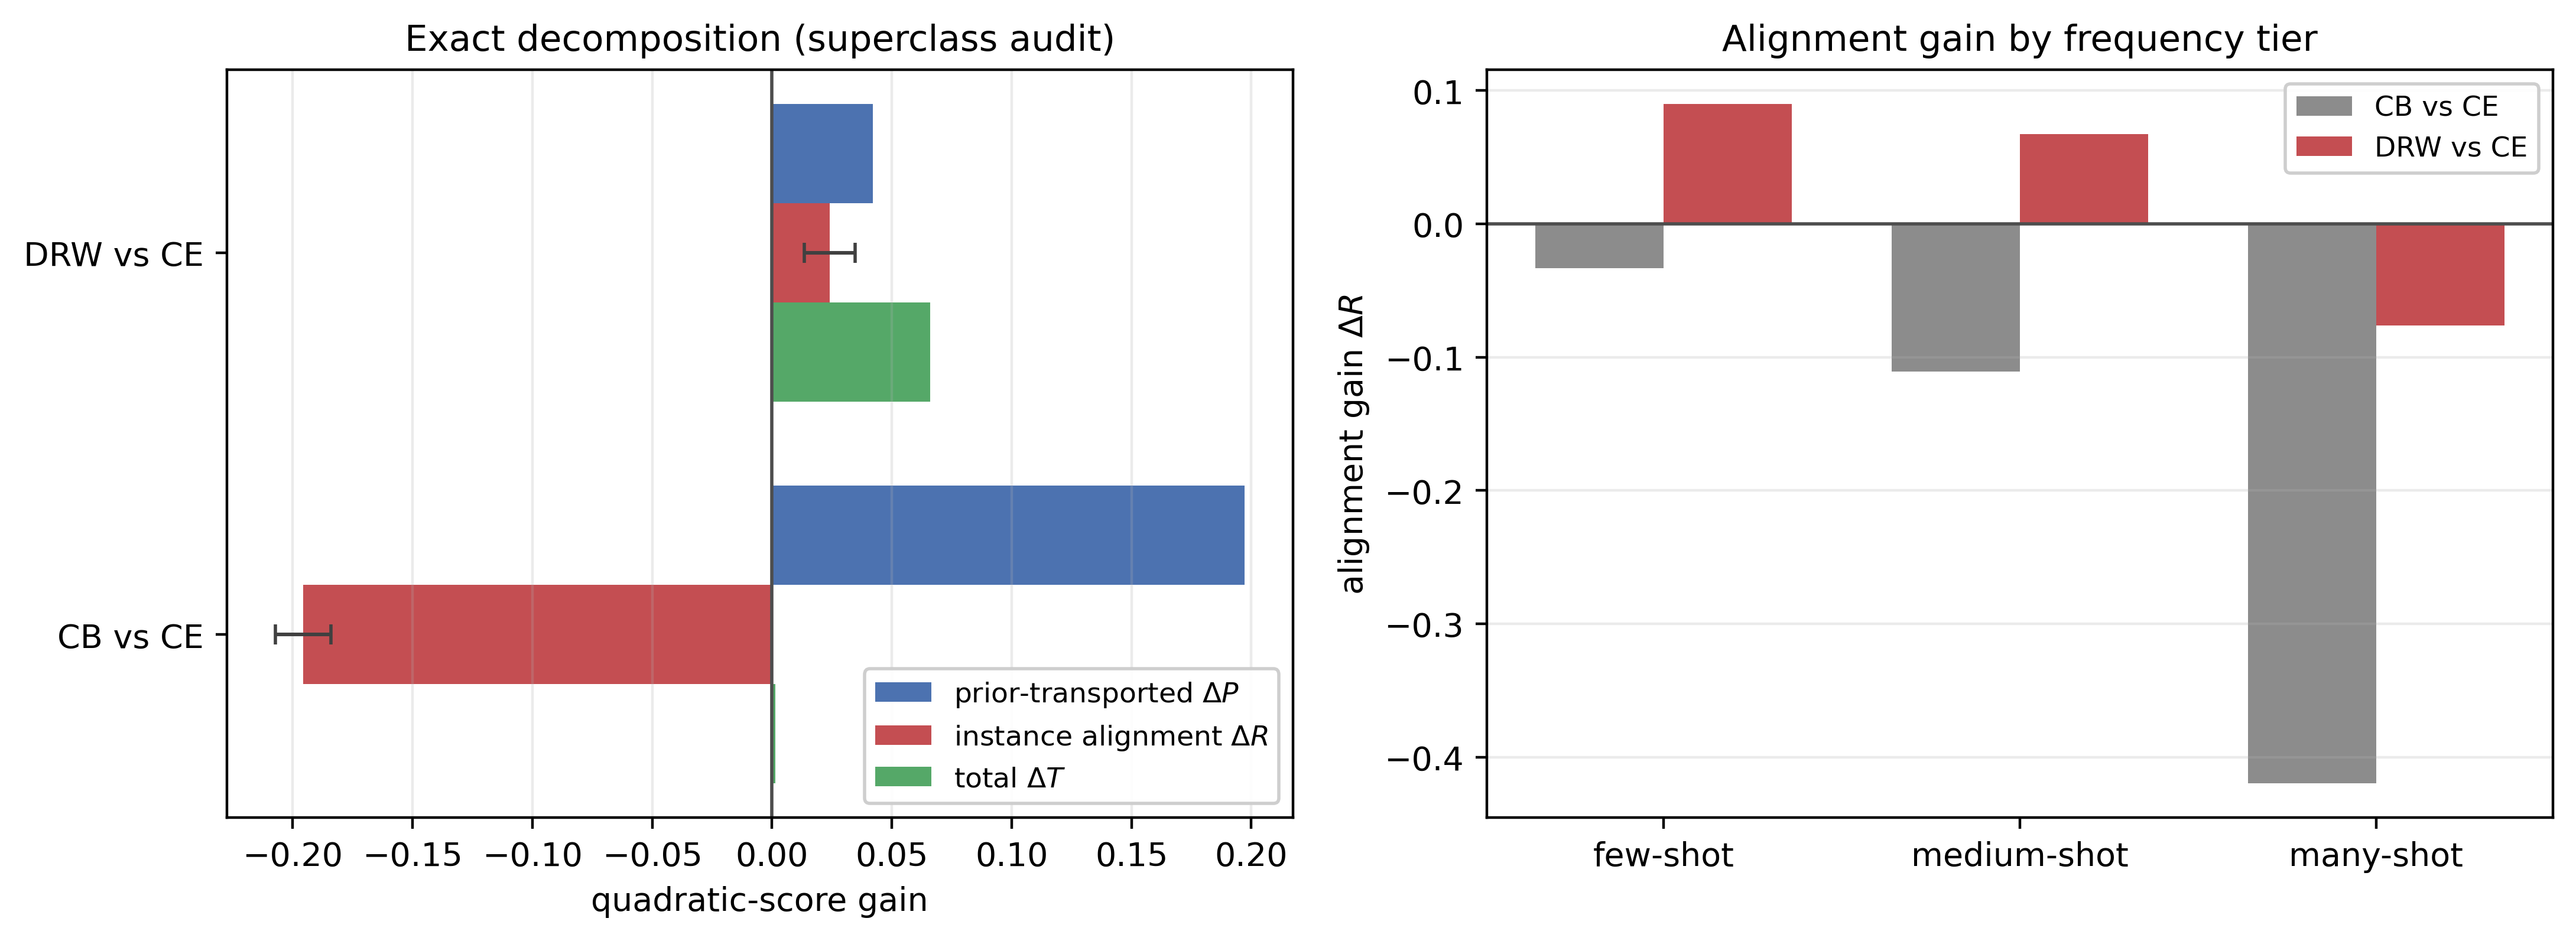
\includegraphics[width=\textwidth]{figures/fig5_cifar_lt.png}
\caption{\textbf{The same attribution transfers to a second task.} Left: exact
decomposition at the superclass audit. The CB total gain (green) is visually almost
absent at $+0.00143$ while its two channels reach $\pm0.2$ -- a near-zero aggregate
score concealing two large opposing effects. DRW's smaller total is genuinely split
between both channels. Error bars are 95\% H\'ajek intervals on $\widehat{\Delta R}$.
Right: the covariance channel by training-frequency tier, showing that DRW's genuine
per-instance gain is concentrated on rare classes and negative on the head.}
\label{fig:cifar}
\end{figure*}

Coarsening behaves as Proposition~\ref{prop:coarsen} predicts. Moving from the 20
superclass cells to a single global cell changes the credited covariance from $-0.19569$
to $-0.25430$; the difference is the between-cell covariance term, which is negative
here, so the coarse audit overstates the covariance loss by attributing to it structure
that the superclass partition correctly assigns to $\Delta P$. The finer partition is
again the conservative reading, for the same reason as in Section~\ref{sec:ablations}
and now in a second domain.

\subsection{Long-tailed text classification}\label{sec:textlt}

Sections~\ref{sec:results}--\ref{app:lt} test two vision tasks that share cached
probability vectors and grouping variables grounded in class frequency or object geometry.
To test the breadth Section~\ref{sec:broader} claims -- any benchmark supplying two
models' full probability vectors, labels, and a declared discrete grouping variable -- we
apply the identical estimator, unmodified, to document category prediction on 20
Newsgroups \citep{lang1995newsweeder}. Neither the predictors nor the grouping variable are
visual here: documents replace images, and the declared $\phi$ is a topical grouping
rather than a spatial or class-frequency one, so a favorable result cannot be attributed
to anything specific to vision data.

We build a long-tailed training subset with the same exponential profile as
CIFAR-100-LT (imbalance ratio $100$, Section~\ref{app:lt}), applied to 20
Newsgroups' 20 fine categories, keeping the standard balanced test split ($7{,}532$
documents) untouched (Appendix~\ref{app:implementation}). The 20 categories fall into
six conventional coarse topics -- computing, recreation, science, politics, religion,
and classifieds -- which we use as the primary declared $\phi$, the direct analogue of
CIFAR's coarse superclasses; a global (trivial) and a training-frequency-tier partition
are reported alongside, as in Section~\ref{app:lt}. Documents are represented by a
TF-IDF vector reduced to $300$ dimensions by truncated SVD, and the three compared
classifiers -- CE, CB, and DRW -- follow the same three-arm protocol as
Section~\ref{app:lt}: an identical small MLP architecture and optimizer across runs,
differing only in per-example loss weight (Appendix~\ref{app:implementation}). Test
documents are independent units, so the plain H\'ajek interval of Section~\ref{sec:inference}
applies directly, as for CIFAR.

\paragraph{Result.} Table~\ref{tab:textlt} decomposes both re-weighting schedules' gain
over the cross-entropy baseline (top-1 accuracies $0.3532$ CE, $0.3960$ CB, $0.3776$
DRW). The two schedules land in opposite channels here, which is itself the finding
worth reporting: on this task it is class-balanced re-weighting from initialization, not
the deferred schedule, that buys genuine within-topic covariance gain ($+0.04317$, CI
$[0.03664,0.04970]$, $37.9\%$ of its total gain), while DRW's comparably sized total gain
($0.11490$ vs.\ CB's $0.11388$) is $98.6\%$ transported, its residual covariance
statistically indistinguishable from zero at the superclass audit ($+0.00155$, CI
$[-0.00296,0.00605]$, $p=.236$) and significantly negative once the coarser tier
partition is used instead ($-0.00901$, CI $[-0.01428,-0.00374]$). This is the reverse of
Section~\ref{app:lt}'s image-classification finding, where CB's near-zero total
masked a large covariance-gain \emph{loss} and DRW's gain was genuinely covariance-driven.
Nothing about the estimator or the construction of $\phi$ changed between the two
applications; what changed is which training recipe, on which data, buys real
per-instance discrimination -- exactly the composition question an aggregate score or an
accuracy difference alone cannot answer, now demonstrated on a domain with neither a
class-frequency table nor a spatial prior.

Coarsening moves both comparisons in the direction Proposition~\ref{prop:coarsen} allows
without requiring: CB's credited covariance falls from $0.04317$ at the superclass
partition to $0.04185$ at the global cell and $0.03578$ at the tier partition, while
DRW's changes sign twice, from a small positive residual (superclass) to a small
negative one (global) to a significant negative one (tier). None of these differences
overturns CB's conclusion, but DRW's illustrates exactly why the finest defensible
partition is the conservative default (Section~\ref{sec:coarsening}): a reader stopping
at the coarser tier partition would report a significant covariance \emph{loss} for a
method whose finer-grained residual is not distinguishable from zero.

\begin{table}[t]
\centering
\caption{WAGER decomposition on the 7,532-document balanced 20-Newsgroups-LT test
split. Gains use the quadratic score; CI is the (unclustered) H\'ajek interval on
$\widehat{\Delta R}$, documents being independent units; $p$ is the 499-shift
randomization diagnostic, one-sided for a positive covariance gain.}
\label{tab:textlt}
\resizebox{\textwidth}{!}{%
\begin{tabular}{@{}llrrrr@{}}
\toprule
Comparison & Audit cell $\phi$ & $\widehat{\Delta T}$ & $\widehat{\Delta P}$ &
$\widehat{\Delta R}$ (95\% CI) & $p$ \\
\midrule
CB vs CE  & superclass (6) & $0.11388$ & $0.07071$ & $0.04317\,[0.03664,0.04970]$ & $.002$ \\
CB vs CE  & global (1)     & $0.11388$ & $0.07203$ & $0.04185\,[0.03381,0.04990]$ & $.002$ \\
CB vs CE  & tier (3)       & $0.11388$ & $0.07810$ & $0.03578\,[0.02825,0.04331]$ & $.002$ \\
\midrule
DRW vs CE & superclass (6) & $0.11490$ & $0.11335$ & $0.00155\,[-0.00296,0.00605]$ & $.236$ \\
DRW vs CE & global (1)     & $0.11490$ & $0.11809$ & $-0.00319\,[-0.00884,0.00245]$ & $.980$ \\
DRW vs CE & tier (3)       & $0.11490$ & $0.12391$ & $-0.00901\,[-0.01428,-0.00374]$ & $1.000$ \\
\bottomrule
\end{tabular}
}
\end{table}

\begin{figure*}[t]
\centering
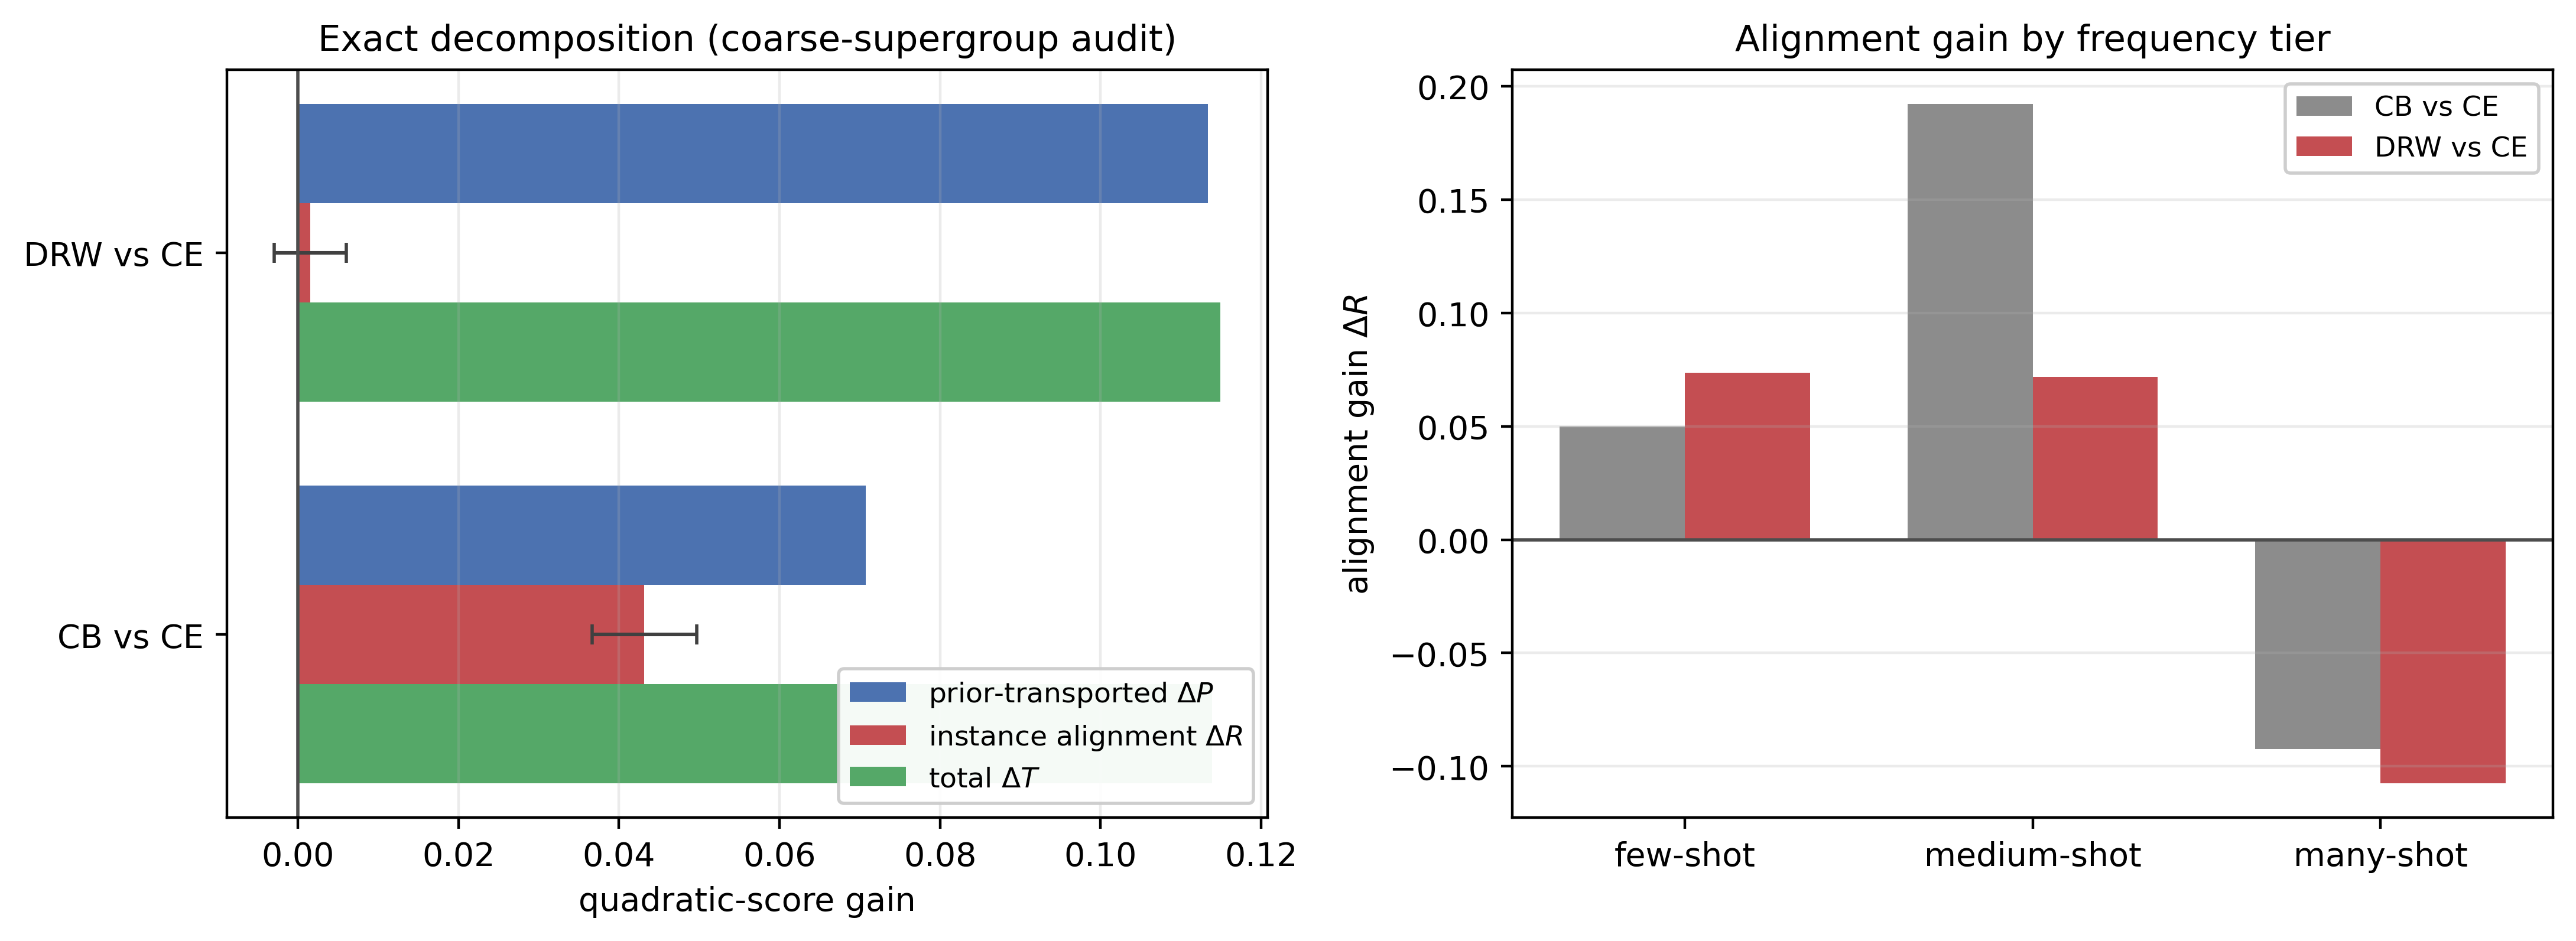
\includegraphics[width=\textwidth]{figures/fig8_text_lt.png}
\caption{\textbf{A third domain, with neither a spatial nor a class-frequency prior.}
Left: exact decomposition at the coarse-topic audit; CB's total gain is genuinely split
between both channels while DRW's is almost entirely transported. Error bars are
95\% H\'ajek intervals on $\widehat{\Delta R}$. Right: covariance gain by
training-frequency tier for both schedules, showing the same head-loses/tail-gains
signature as Figure~\ref{fig:cifar} despite the change of domain and grouping variable.}
\label{fig:textlt}
\end{figure*}

Table~\ref{tab:textlt-tier} breaks the superclass-audit covariance down by
training-frequency tier for both schedules; the two methods agree in shape even though
their superclass totals diverge sharply in composition, each gaining covariance on rare
and medium-frequency categories and losing it on frequent ones, the same qualitative
signature Section~\ref{app:lt} reports for image classification.

\begin{table}[t]
\centering
\caption{Covariance gain by training-frequency tier at the superclass audit,
20-Newsgroups-LT. Both schedules gain within-group covariance on rare and medium categories
and lose it on frequent ones.}
\label{tab:textlt-tier}
\begin{tabular}{@{}lrrr@{}}
\toprule
Tier & $n$ & $\widehat{\Delta R}$, CB vs CE & $\widehat{\Delta R}$, DRW vs CE \\
\midrule
Few-shot ($<20$)          & 1954 & $0.04991$  & $0.07352$  \\
Medium-shot ($20$--$100$) & 2610 & $0.19213$  & $0.07171$  \\
Many-shot ($>100$)        & 2968 & $-0.09227$ & $-0.10753$ \\
\bottomrule
\end{tabular}
\end{table}

This third domain uses a single trained pair per schedule rather than the multi-seed,
calibration-matched protocol Section~\ref{app:lt} applies to CIFAR-100-LT; extending
that fuller protocol to text is the natural next replication, not a step this section
claims to have taken.
